\documentclass[UTF8]{ctexart}
\usepackage[a4paper,left=3cm,right=3cm,top=2cm]{geometry}
\usepackage{amsmath}
\usepackage{enumitem}
\usepackage{float}
\usepackage{threeparttable}
\usepackage{caption}
\usepackage{multirow}
\usepackage{graphicx}
\usepackage{listings}
\usepackage{xcolor}
\usepackage{amssymb}
\renewcommand{\figurename}{Figure}
\definecolor{dkgreen}{rgb}{0,0.6,0}
\definecolor{gray}{rgb}{0.5,0.5,0.5}
\definecolor{mauve}{rgb}{0.58,0,0.82}

\lstset{frame=tb,
  language=C++,
  aboveskip=3mm,
  belowskip=3mm,
  showstringspaces=false,
  columns=flexible,
  basicstyle={\small\ttfamily},
  numbers=left,%设置行号位置, none不显示行号
  numberstyle=\tiny\courier, %设置行号大小
  numberstyle=\tiny\color{gray},
  keywordstyle=\color{blue},
  commentstyle=\color{dkgreen},
  stringstyle=\color{mauve},
  breaklines=true,
  breakatwhitespace=true,
  escapeinside=`,%逃逸字符(1左面的键),用于显示中文例如在代码中`中文...`
  tabsize=4,
  extendedchars=false %解决代码跨页时,章节标题,页眉等汉字不显示的问题
}

\setlength\lineskiplimit{5.25bp}
\setlength\lineskip{5.25bp}

\title{Lab07 Report}
\author{崔士强 PB22151743}
\date{January 12, 2024}

\bibliographystyle{plain}

\begin{document}

\maketitle
This lab is completed in MacOS.

\section{Purpose}
The purpose of the program is to implement a simple LC-3 assembler in C++.

Anticipated outcomes: A \lstinline{.txt} file including the machine language code translated from the input \lstinline{.asm} file

\section{Principles}
\subsection{Two-pass process}
The assembling process is a two-pass process. The first pass reads the labels and creates a symbol table.
The second pass reads the code and translate it into the machine language. 

In order to identify the labels, a vector including all the operations is generated: \lstinline{vector<string> instSet}.
 If a line is not started with an operation, store the first word as a label in the map \lstinline{map<string, int> symbol_table}.

In the second pass, the code is translated into machine language line by line:
\begin{lstlisting}
  PC = 0;
  for(const auto &line : lines){
      if(line == ".END") continue;
      PC++;
      output_lines.push_back(translate_instruction(line, symbol_table, instSet, PC));       
              // Translate the instruction in the second pass
  }
\end{lstlisting}

The \lstinline{PC} here is not the value of program counter. It started with 1 in order to simplify the process.

\subsection{Translation}
After identifying the operation, the translation process can be broken up into three parts:
\begin{enumerate}
  \item Registers
  \item Immediate values
  \item Labels
\end{enumerate}

For each of them, a function is defined:
\begin{lstlisting}
  void FetchRegister(string &instruction, string &machine_code);
  void FetchImmediate(string &instruction, string &machine_code, const int len);
  void FetchLabel(string &instruction, string &machine_code, const map<string, int> symbol_table, const int PC, const int offset_length);
\end{lstlisting}

For registers and immediate values, the work is mainly converting strings of decimal or hexadecimal numbers to fixed-length strings of binary numbers. 
And for labels it's mainly computing offsets.

\section{Procedure}
\subsection{Bugs encountered}
During execution, I found that negative numbers could not be converted to 2's complement binary representation
correctly. The reason was that the '$-$' before a number was not deleted. So sign-extending this number would 
give a result like \lstinline{------110}.

Solution: add the following code:
\begin{lstlisting}
  if(s[0] == '-'){
        negative = true;
        s.erase(0, 1);
    }
\end{lstlisting}
\subsection{Chanllenges}
Given that: 
\begin{enumerate}
  \item I've never learned C++ before.
  \item Implementation using C is more complex due to the absence of useful libraries like STL.
\end{enumerate}

A major challenge in this lab is getting familiar with C++. If given more time, maybe I'll try using regex, which could simplify the work.

\section{Results}
Results are shown below:
\begin{lstlisting}[caption = test\_in.asm]
  .ORIG x3000
  MAIN LD R1, DATA
  TEST ADD R1, R1, #-10
  BRZP TEST
  ST R1, MEM
  TRAP x25
  DATA .FILL x1234
  MEM .BLKW #2
  .STRINGZ "HelloWorld1337"
  .END
\end{lstlisting}

\begin{figure}[H]
  \centering
  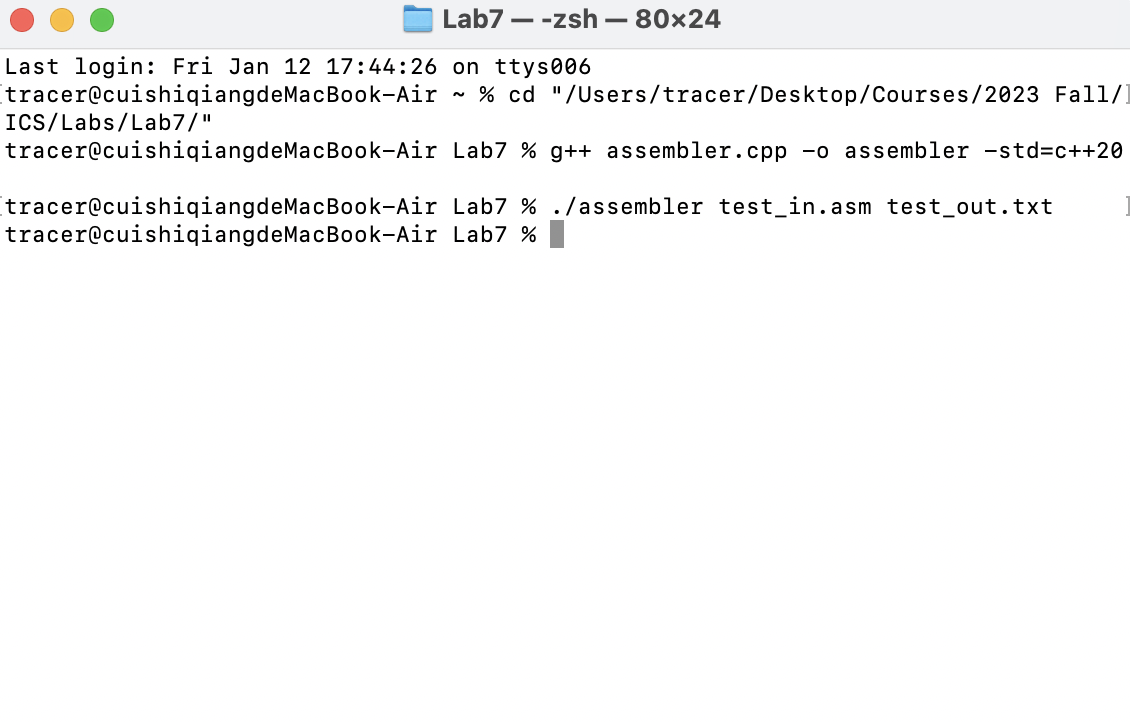
\includegraphics[scale=0.4]{command.png}
  \caption{Command}
\end{figure}

\begin{figure}[H]
  \centering
  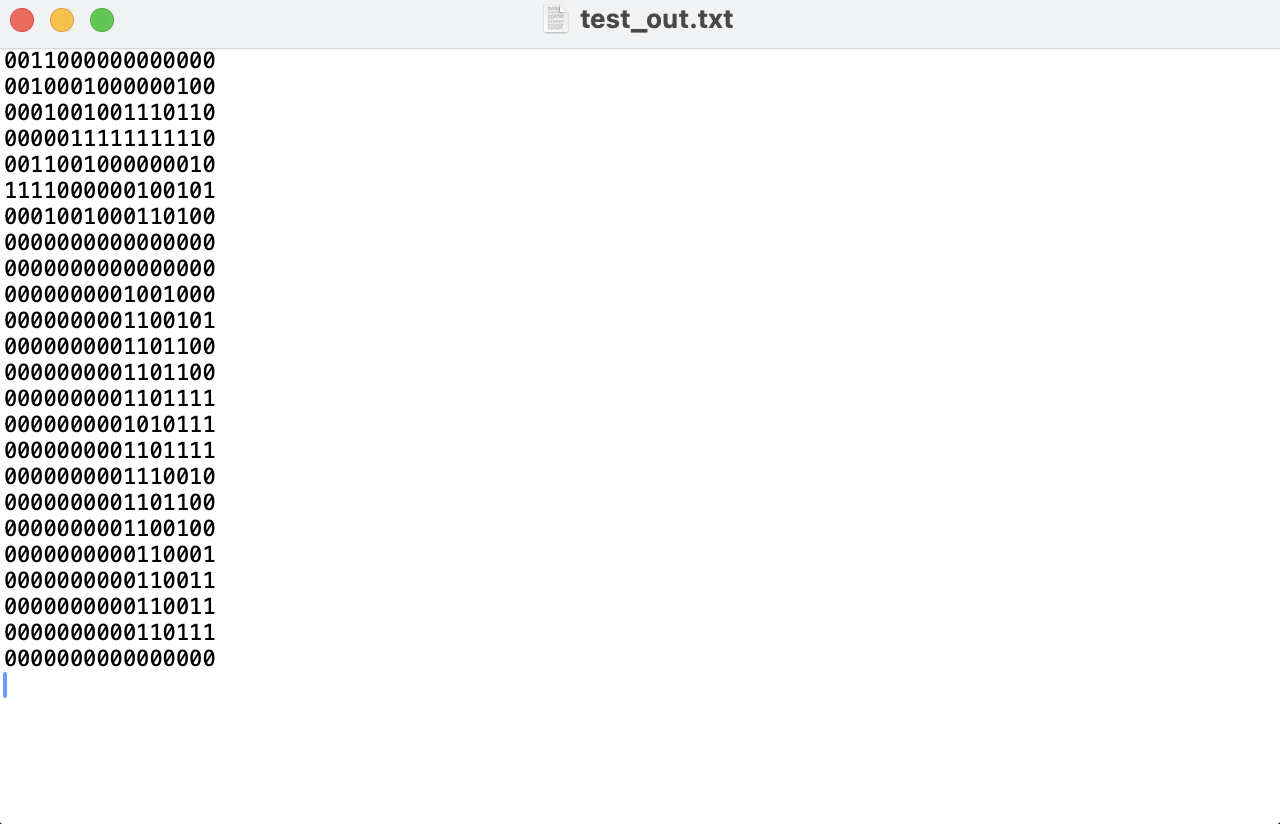
\includegraphics[scale=0.4]{result.png}
  \caption{Result}
\end{figure}

\begin{figure}[H]
  \centering
  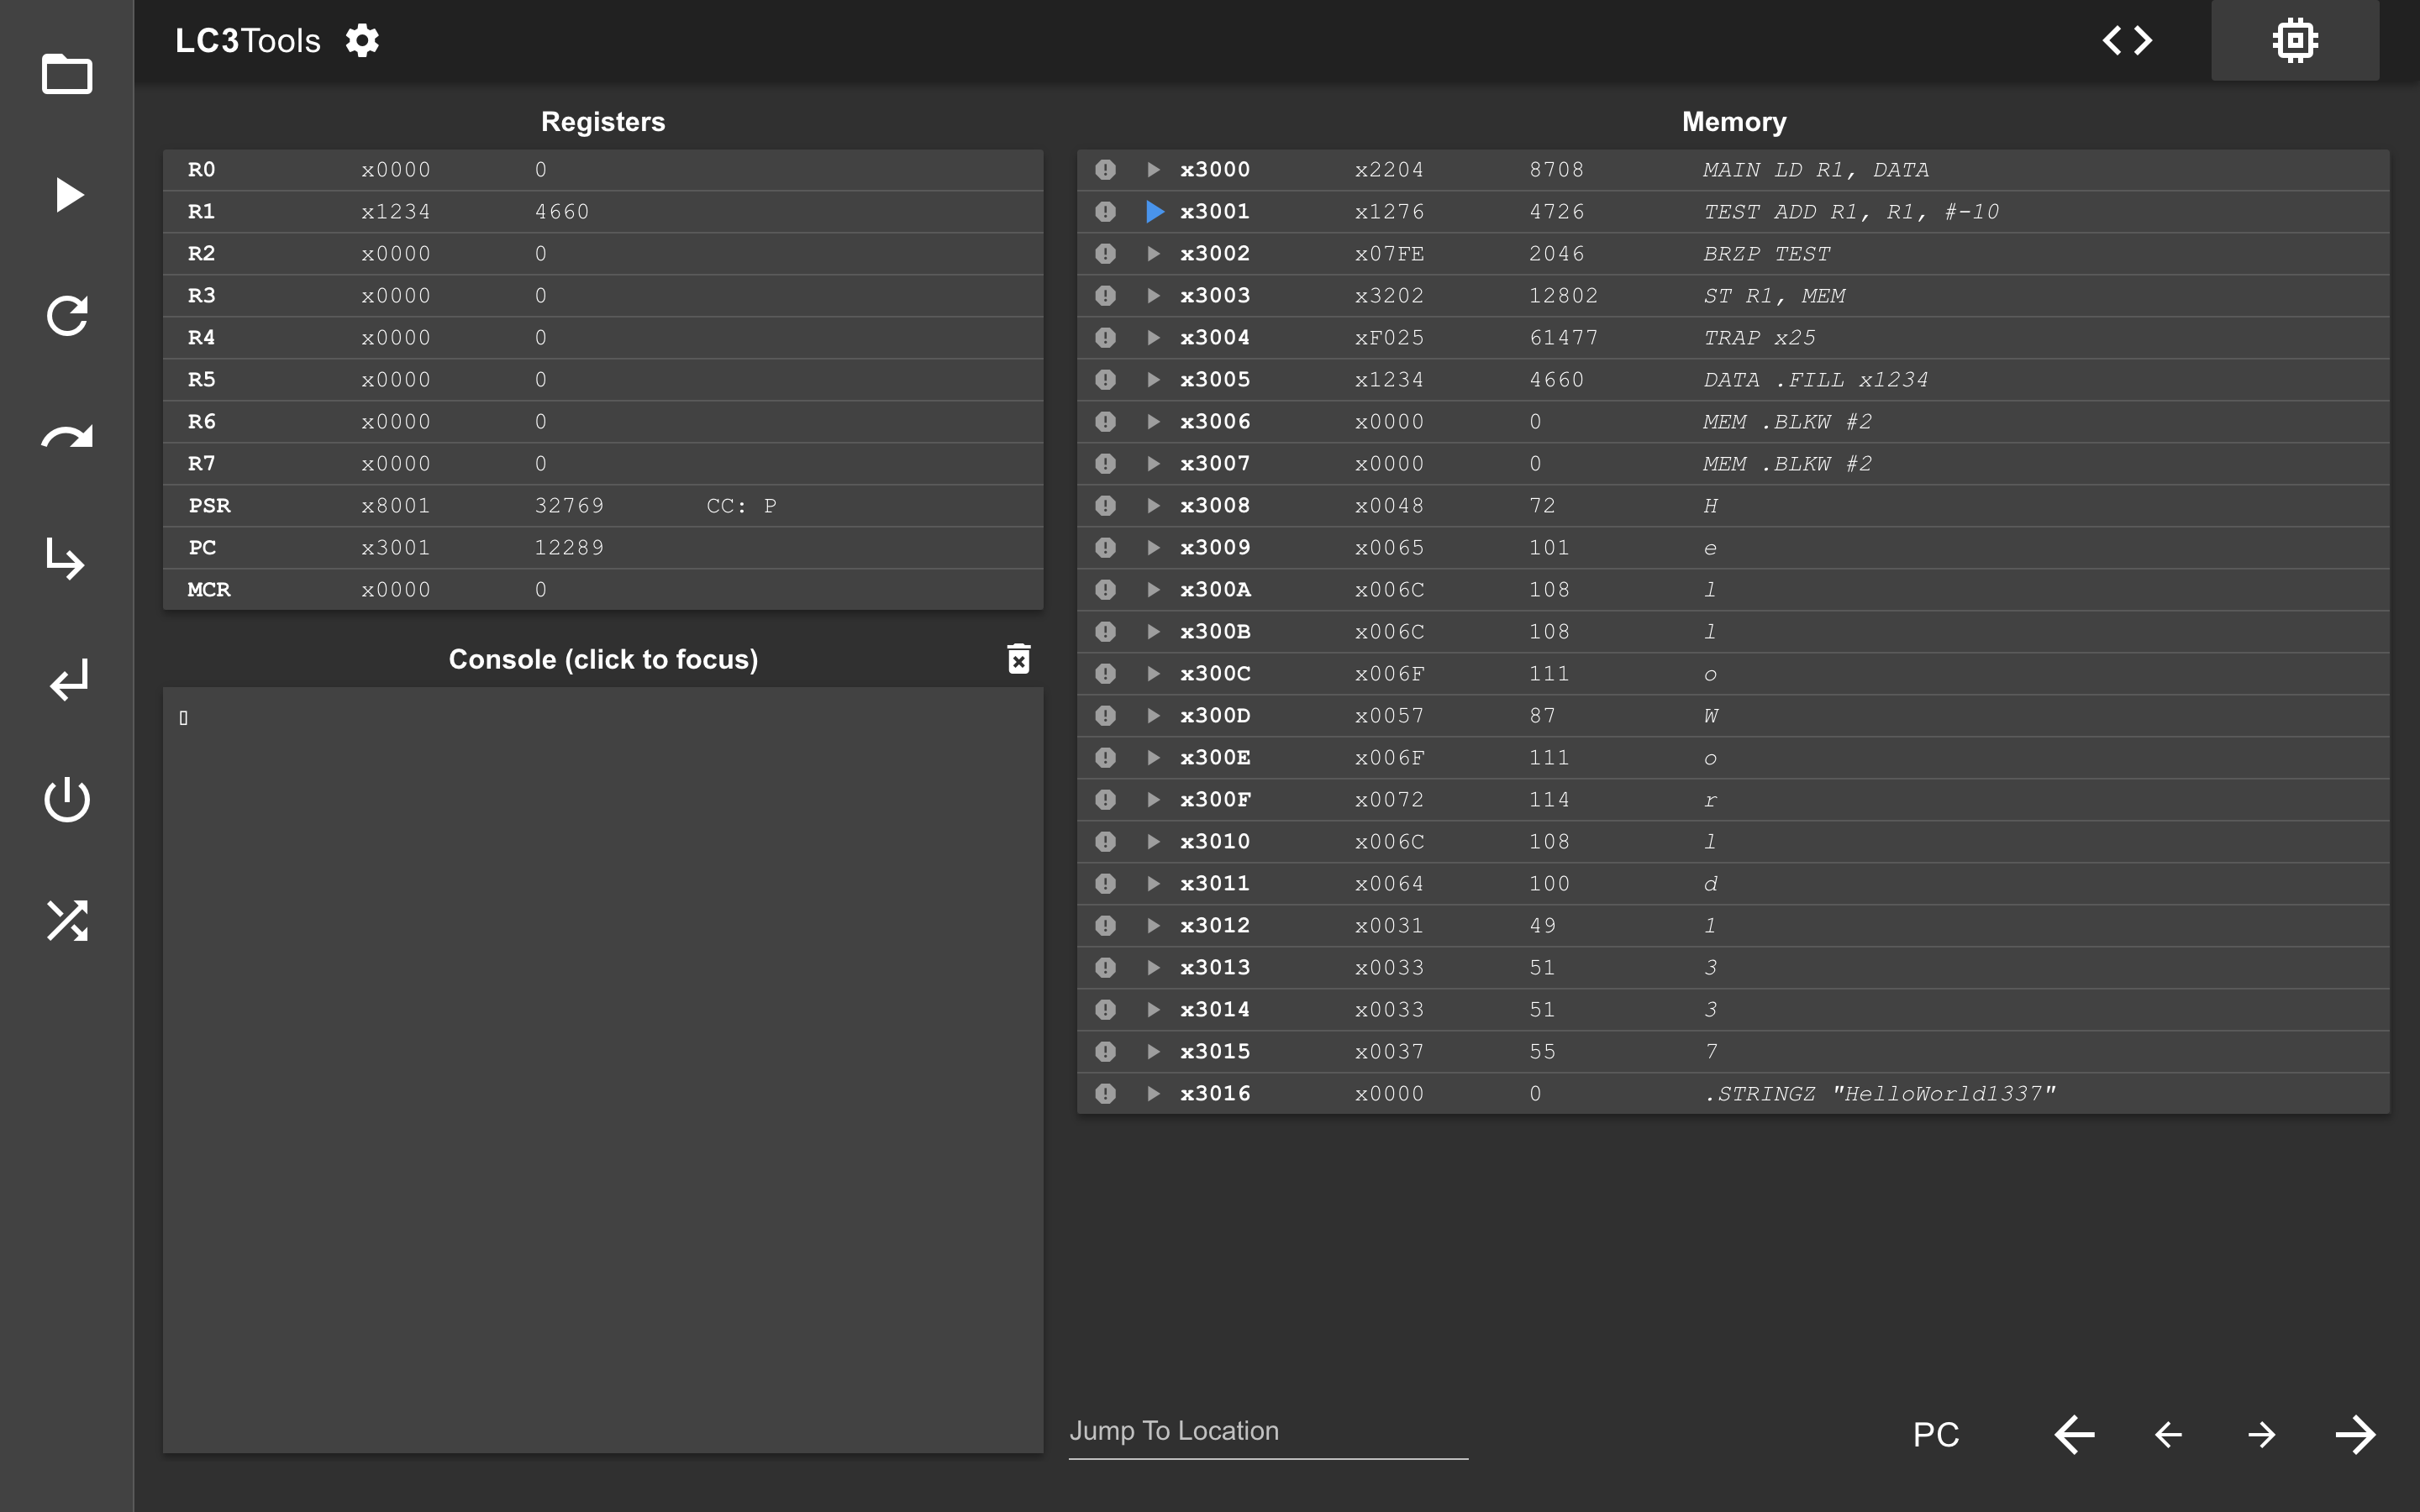
\includegraphics[scale=0.25]{lc3.png}
  \caption{Assembly result in LC-3 Tools}
\end{figure}

The machine code in output file is correct.

\bibliography{math}

\end{document}
\iffalse
\begin{figure}[H]
    \centering
    \includegraphics[scale=0.5]{name.png}
    \caption{name}
\end{figure}
\fi
